\documentclass[a4paper]{article}

\usepackage[margin=1in]{geometry}
\usepackage{graphicx}
\usepackage{parskip}
\usepackage[cache=false]{minted}
\usepackage{amsmath}
\usepackage[width=0.8\textwidth]{caption}

\setminted[python] {
    linenos,
    frame=single,
    fontsize=\footnotesize,
    tabsize=4, 
    breaklines
}

\title{\vspace{-5ex}COMP6223 Coursework 1\\Hybrid Images}
\date{8 Nov.\ 2018}
\author{Rhys Thomas, \tt{rt8g15@ecs.soton.ac.uk}}

\begin{document}
\maketitle

\section{Template Convolution}
Template convolution is a group operator used to modify pixels in an image. Methods of performing the convolution include either an iterative approach, walking through the image and multiplying/summing neighbouring pixels, or using the Fourier transform.
 
\subsection{Iterative Method}
The iterative method works by multiplying every image pixel within a kernel and then summing them together. This is quite computationally expensive since the number of iterations over the image is given by equation~\ref{eq:iterative}.

\begin{equation}
    \mbox{\# of Iterations} = \prod_{i\in\{h,w\}}\left(\mbox{Image}_i-\left\lfloor\frac{\mbox{Kernel}_i}{2}\right\rfloor\right)\times\mbox{Colours}
    \label{eq:iterative}
\end{equation}

So for a $300\times 300$ tricolour image with a kernel size of $3\times 3$, this would result in 268,203 iterations! The source code for this method is given below.

\inputminted[
    firstline = 35,
    lastline = 61
]{python}{../hybrid.py}

An artefact intrinsic to the iterative method is that the resulting image needs to be cropped. This is because the kernel has a border which is not included in the calculation, thus reducing the size of the image. The effect of this is shown in figure~\ref{fig:no-crop}.

\begin{figure}
    \centering
    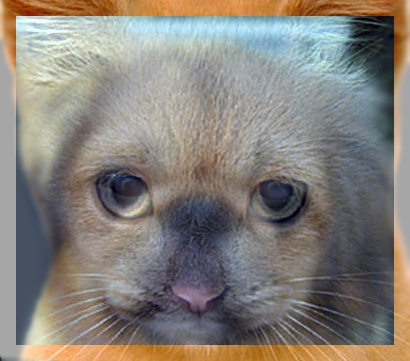
\includegraphics[width=0.25\textwidth]{../no_crop}
    \caption{Template convolution without cropping.}
    \label{fig:no-crop}
\end{figure}

Both this and the computation expense of the operation gives rise to the need for alternative methods. Performing convolution via the Fast Fourier Transform removes the padding border around the image -- since the kernel is padded to the image size -- and is much faster than iterative calculations.

\subsection{Fourier Method}
The Fourier convolution gives an equivalent result to template convolution, except it is more computationally efficient by working in the frequency domain, rather than the spacial domain. 

The image and kernel is first loaded and their dimensions examined. With this information we are able to calculate the padding required around the kernel to make it the same dimensions as the (larger) image. 

When applying convolution using Fourier, the kernel and image must be the same size. This was not a requirement for the iterative method, since it scanned across the image applying calculations on groups of pixels. The padding can be easily calculated by subtracting the kernel dimensions from that of the image, and floor-dividing (\texttt{//}) by 2. Padding around the kernel is set to zero.

The template is then flipped in the spacial domain, this is to insure that we are implementing \textit{convolution} rather than \textit{correlation}, which does not require spacial domain inversion. The Fourier convolution is then calculated for each colour channel in the image using equation~\ref{eq:fft}. 

\begin{equation}
    \mathcal{F}^{-1}\left( \mathcal{F}(\mbox{image}) \cdot\times \mathcal{F}(\mbox{template})\right) \label{eq:fft}
\end{equation}

The complete algorithm for the Fourier convolution is shown below.

\inputminted[
    firstline = 64,
    lastline = 88
]{python}{../hybrid.py}

It can be seen on line 85 that after computing the inverse FFT, \texttt{fftshift()} is called. This is due to how numpy calculates the two dimensional FFT; it assumes the origin (DC components) are at the top left of the image whereas we define them in the centre. To compensate for this, we manually shift the FFT so that the origin is in the centre of the image, which gives us the desired result. The effect of this shifting can be seen in figure~\ref{fig:no-shift}, pixels that exceed the image dimensions wrap around to the opposite side.

\begin{figure}[!htbp]
    \centering
    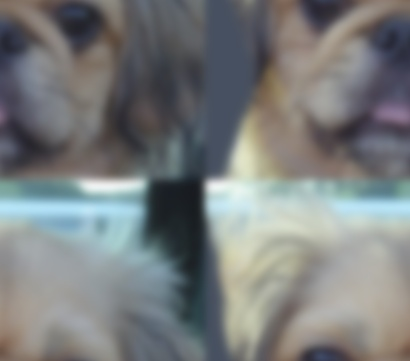
\includegraphics[width=0.25\textwidth]{../no_shift}
    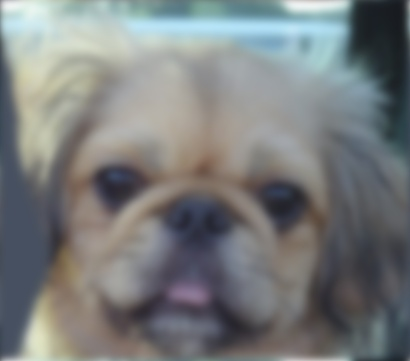
\includegraphics[width=0.25\textwidth]{../low}    
    \caption{Effect on the image when not shifting (left) and shifting (right) the convolved FFT.}
    \label{fig:no-shift}
\end{figure}

The speed difference between the iterative (``brute-force'') and Fourier methods is noticeable when you run the script, and the recorded execution times for each are as follows,

\begin{minted}[
    frame=single,
    fontsize=\footnotesize,
    tabsize=4
]{text}
time ./hybrid.py -i data/dog.bmp data/cat.bmp -c 4 4 -o hybrid.jpg -v visual.jpg  
    6.68s user 0.15s system 80% cpu 8.496 total
    
time ./hybrid.py -i data/dog.bmp data/cat.bmp -c 4 4 -o hybrid.jpg -v visual.jpg -f 
    0.67s user 0.13s system 156% cpu 0.510 total
\end{minted}

This emphasises how much more practical/efficient the Fourier method is. Iterative template convolution is useful to \textit{understand} convolution, however it serves little purpose beyond that.

\section{Gaussian Filters}
To low-pass filter an image, convolve a Gaussian filter -- of particular cutoff frequency, $\sigma$ -- with the original image. One can simply subtract the low-pass filtered result from the original image in order to produce the high-pass filter equivalent. 

The equation for a 2-dimensional Gaussian filter is shown in equation~\ref{eq:gaus}, however the $1/2\pi\sigma^2$ term is usually approximated to the sum of the kernel over the window size.

\begin{equation}
    G(x, y, \sigma) = \frac{1}{2\pi\sigma^2}\exp\left(\frac{-(x^2+y^2)}{2\sigma^2}\right)
    \label{eq:gaus}
\end{equation}

The below function creates a Gaussian kernel, based on the value of $\sigma$ passed to the function. 

\inputminted[
    firstline = 91,
    lastline = 114
]{python}{../hybrid.py}

Figure~\ref{fig:high-low} shows the effect of applying a Gaussian blur to an image in order to produce a low-pass filtered version (left). As previously mentioned, a low-pass filtered image can be subtracted from the original image in order to produce a high-pass filtered equivalent (right). Note that each pixel of the high-pass image is increased by \texttt{0.5} to increase visibility.

\begin{figure}[!htbp]
    \centering
    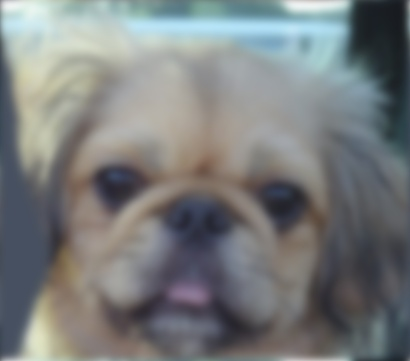
\includegraphics[width=0.25\textwidth]{../low}
    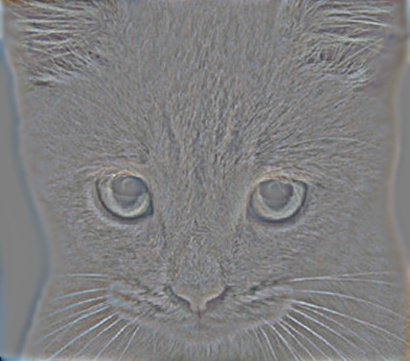
\includegraphics[width=0.25\textwidth]{../high}
    \caption{Low and high-pass filtered images with $\sigma=4$.}
    \label{fig:high-low}
\end{figure}

\section{Hybrid Images}
Hybrid images are formed by summing together two \textit{different} low-pass and high-pass filtered images. The higher frequencies dominate when the viewing distance is short, however at a longer distance the lower frequencies dominate. Figure~\ref{fig:visual} is a hybrid image composed from the two images in the previous section. The result is downsampled in order to demonstrate the aforementioned effect.

\begin{minted}[
    frame=single,
    fontsize=\footnotesize,
    tabsize=4
]{text}
> ./hybrid.py -i data/dog.bmp data/cat.bmp -c 4 4 -o hybrid.jpg -v visual.jpg -f
\end{minted}

\begin{figure}[!htbp]
    \centering
    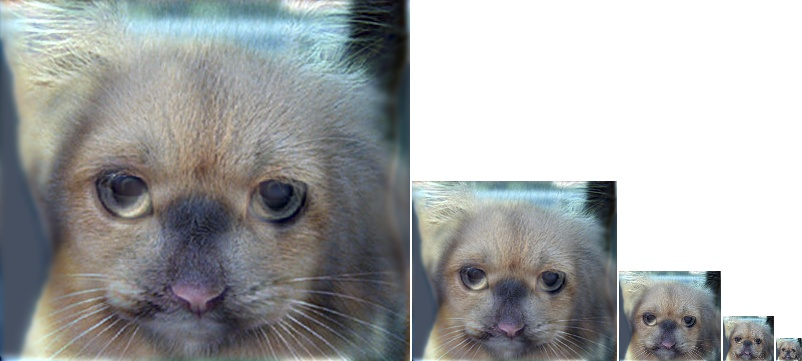
\includegraphics[width=0.75\textwidth]{../visual}
    \caption{Visualising the effect of hybrid images filtered with $\sigma=4$.}
    \label{fig:visual}
\end{figure}

\section{Other Kernels}
To demonstrate the convolution further, the script offers support for additional kernels. You will note that these other convolutions only act on the first image entered with the \texttt{-i} flag. This is to reduce script complexity yet demonstrating the working concept.

\subsection{Sobel Edge Detection}
Sobel edge detection applies the two dimensional kernels shown in the code below. One detects horizontal edges while the other detects vertical edges. The result of these two convolutions can be summed in order to display edges in both directions as shown in figure~\ref{fig:high-low}.

\inputminted[
    firstline = 213,
    lastline = 219
]{python}{../hybrid.py}

This kernel can be applied to the first image in the two element list using the \texttt{-s} flag, as shown below.

\begin{minted}[
    frame=single,
    fontsize=\footnotesize,
    tabsize=4
]{text}
> ./hybrid.py -i Data/plane.bmp Data/bird.bmp -s
\end{minted}

\begin{figure}[!htbp]
    \centering
    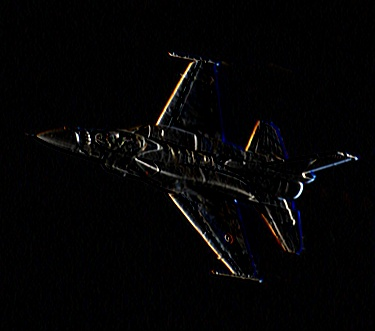
\includegraphics[width=0.25\textwidth]{../sobel_x}
    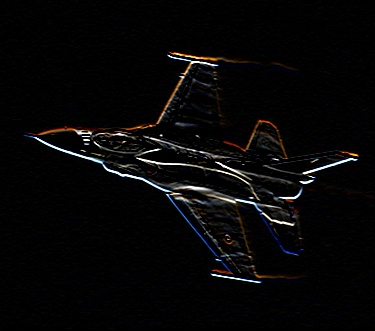
\includegraphics[width=0.25\textwidth]{../sobel_y}
    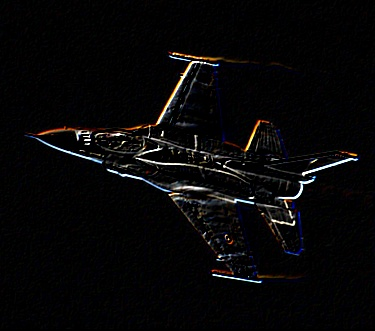
\includegraphics[width=0.25\textwidth]{../sobel_xy}    
    \caption{Sobel edge detection applied in both horizontal (left) and vertical (middle) directions. These are then summed to produce a combined edge detection (right).}
    \label{fig:high-low}
\end{figure}

\subsection{Arbitrary Averaging}
The \texttt{-k} flag allows you to set the dimensions of a simple averaging kernel. The kernel is simply an array of ones, divided by the product of the dimensions specified -- with an additional scaling of 255 for increased display visibility. 

\inputminted[
    firstline = 195,
    lastline = 195
]{python}{../hybrid.py}

Within the \texttt{main} function, the template convolution is used for arbitrary kernels to help demonstrate the effect of asymmetric dimensions on the image border. Notice how the top/bottom borders in figure~\ref{fig:arb-kern} are larger than the left/right.

\begin{minted}[
    frame=single,
    fontsize=\footnotesize,
    tabsize=4
]{text}
> ./hybrid.py -k 31 3 -i Data/bird.bmp Data/plane.bmp -o arb.jpg
\end{minted}

\begin{figure}[!htbp]
    \centering
    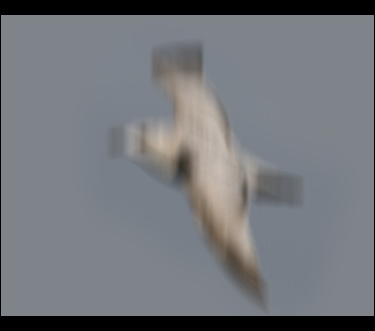
\includegraphics[width=0.25\textwidth]{../arb}
    \caption{Simple averaging with a kernel size of $31\times 3$.}
    \label{fig:arb-kern}
\end{figure}

\section{Usage}
The \texttt{argparse} python module was used to generate arguments for the script. It allows the user to define kernel sizes, cutoff frequencies and input images etc.

\begin{minted}[
    frame=single,
    fontsize=\footnotesize,
    tabsize=4
]{text}
usage: hybrid.py [-h] -i IMAGE IMAGE [-k KERNEL KERNEL] [-c CUTOFF CUTOFF]
                 [-o OUTPUT] [-v VISUAL] [-f] [-s]

optional arguments:
  -h, --help            show this help message and exit
  -i IMAGE IMAGE, --image IMAGE IMAGE
                        Path to input images.
  -k KERNEL KERNEL, --kernel KERNEL KERNEL
                        Kernal size, e.g. 5 7. Note: first image in list will
                        be used.
  -c CUTOFF CUTOFF, --cutoff CUTOFF CUTOFF
                        Gaussian cutoff frequencies, e.g. 5 5.
  -o OUTPUT, --output OUTPUT
                        Path to output image file.
  -v VISUAL, --visual VISUAL
                        Path to output visualisation file.
  -f, --fourier         Use Fourier convolution.
  -s, --sobel           Run Sobel edge detection on the first image.
\end{minted}

Example usage is shown below, with the convolution taking place between ``dog.bmp'' and ``cat.bmp'' with the cutoff frequency of $\sigma=4$ for each. The output hybrid image is saved to ``hybrid.jpg'' and the visualisation is saved to ``visual.jpg''. The \texttt{-f} flag indicates that the Fourier method of convolution will be used.

\begin{minted}[
    frame=single,
    fontsize=\footnotesize,
    tabsize=4
]{text}
> ./hybrid.py -i data/dog.bmp data/cat.bmp -c 4 4 -o hybrid.jpg -v visual.jpg -f
[Data/dog.bmp]	Generating low pass image...
[Data/dog.bmp]	Calculating Gaussian kernel...
./hybrid.py:85: ComplexWarning: Casting complex values to real discards the imaginary part
  output[:, :, colour] = np.fft.fftshift(np.fft.ifft2(Fi * Fk)) / 255
[Data/cat.bmp]	Generating high pass image...
[Data/cat.bmp]	Calculating Gaussian kernel...
Creating hybrid image...
Creating visualisation...
Done.
\end{minted}

\end{document}